\ifdefined\included
\else
\setcounter{chapter}{4} 
\dominitoc
\faketableofcontents
\fi

\chapter{User Study to evaluate an integrated plan and execution scheme in simulation}
\chaptermark{User Study to evaluate an integrated plan and execution scheme in simulation}
\label{chap:5}
\minitoc

\section{Introduction}

why simulation: HRI rebuttal: we rely on a reactive execution, real life robot are slow and not very reactive thus may bias our results

Thus, we developed an interactive simulator running robot policies generated as explained the Chapter~\ref{chap:4}. Then, we conducted a user study using this simulator to evaluate our approach.
First, the simulator is described (planning and exec part). Then, the Procedure of the Study is presented. Eventually, the obtained results are presented and then discussed.

\section{Related work}
of plan+execution, simulator

\section{Interactive Simulator}
planning is same

execution is based on model of execution and mock components

human collaborates in real time with robot in blockwords task

describe simulator, mouse, robot and human capabilities, goal shown, prompt

Synchronization, internal communication through simulated visual signal, explicit reaction time, ID phase currently always successful a success rate can be given. 


***********

In this section we provide a few functional and technical details about the developed interactive simulator used for the User Study.

First, it is using Gazebo to simulate the scene (table, cubes, agents). 
The robot is a Tiago robot from PAL Robotics. We used a MoveIt controller to plan and execute arm motions. We used a publicly available component to control the gaze of the robot. The head behavior is ad hoc and designed by us.
The human agent is simulated only with its hand which is moved with a handmade dedicated controller. 
For simplicity reasons physics of objects isn't simulated, thus, each agent interact with the scene by statically attaching/detaching object respectively to the robot's gripper or the human hand.
A higher level component called the simulator controller is in charge of translating primitive actions to low level commands and calling the previously presented controllers to make the agent perform actions. Since it manages agent's action, it is also in charge of sending simulated visual signals and indicating when a step is over. Indeed, the agents synchronize themselves using simulated visual signals, and not internal signals. That is, when the human starts performing an action, a brief motion planning phase occur before effectively moving the hand, the motion visual signal is sent to the robot only at this moment. Moreover, to simulate some real perception aspect, a voluntary reaction time is introduced in the robot. Thus, the visual signal can be treated only after this reaction time is passed. A step starts when one agent starts acting (the human or the robot) and it is over when both agents are inactive. Hence, once one agent started to act the other is free to perform an action concurrently and the step will be over only when both are done. If the other agent doesn't act it will be considered as passive/inactive and the step will be over as soon as the first agent finishes.

Then we can find the respective agents' components. The robot component is an implemented version of the model of execution. Its purpose is to supervise the policy execution of the robot while running the automaton described in the model of execution. In practice, the robot starts by indicating when the step started with a sound signal. Then, it waits to receive the visual human signals for a defined amount of time. Without any visual signal the human is considered as passive. The human can either start acting (how will be described just after), which will eventually send a visual signal to the robot, or the human can make an explicit hand gesture to indicate to the robot that they will be passive (this doesn't force the human to be passive for the whole step). Note that even if the robot received the human visual signal of the human starting to act, the actual action being performed isn't yet identified, it only means that the human started to act. The robot must perform a dedicated identification process (ID Phase/Process) to identify the human action. We assume that the hand gesture that the human can make is always successfully identified instantly (without ID Process). Once either the signal received or the time-out reached, if the best robot action doesn't depend on the human decision then the robot can directly start executing this action. The robot action choice is sent to the simulator controller that will start executing the action. If the best robot action depends on the human decision then the human decision must be identified and the ID Process is run. Only after the robot can perform the best action indicated by the policy which is compliant with the identified human action. If the ID Process fails then the robot remains passive, this case is already part of the policy.
Eventually the robot waits for the step over signal from the simulator controller and run the Assessment Process. The latter identify what happened during the step (which action the human performed, even if ID wasn't necessary) and in which state we are to be ready to execute the next step and progress in the policy and toward the goal. 

The human action execution consists in the following. First, the gazebo simulator is made as the main Human-Machine Interface (HMI). Through a handmade plugin one can mouse click in the gazebo simulator window. The click position is sent on a ROS Topic and treated in a dedicated node to potentially trigger a human action. For instance, clicking on a cube starts a "picking" action with the corresponding cube as parameter, clicking on the stack area starts a "place" action, clicking on the table while holding a cube starts a "hold" action, and clicking on the hand make an explicit hand gesture to signal the robot the human desire to be passive. After clicking the hand once, the participant can click another time to indicate the robot full passivity until further notice. The robot will consider the human as unavailable or even not present and will not wait for them. 
For this to be possible we did the following. First, another gazebo plugin has been written to lock the GUI camera as a First Person View and avoid the participant to accidentally move the camera.
Then, at every step, the robot component sends to the component receiving the coordinates of the click the currently valid human actions that the participant can perform. Thus, the participant cannot try to place a cube without holding it. Eventually, each human action is mapped to a clickable zone on the gazebo window. Hence, when the click coordinates are received, we check if it is inside one of the designed zone and is the action associated to the zone is currently valid. If so, then the action decision is sent to the simulator controller to be executed. 
For clarification purpose, when clicking on a cube the robot doesn't immediately know that the human is picking a cube. First, it will know that the human started to act only after receiving the visual signal (after the defined reaction time). And the robot must perform an additional perception phase (ID Process) to identify which action the human performed. 

Additionally, a small prompt overlay is present to simulate a potential screen with which the robot can communicate its intention to the human during the collaboration.  

Thanks to all these processes, the participant is able to intuitively perform actions using mouse control and can collaborate with the robot to solve the task.

An integrated tutorial has been made to familiarize the participant with the mouse control and the relevant concepts used in the collaboration (notion of step, able to be passive). 

\begin{figure}
    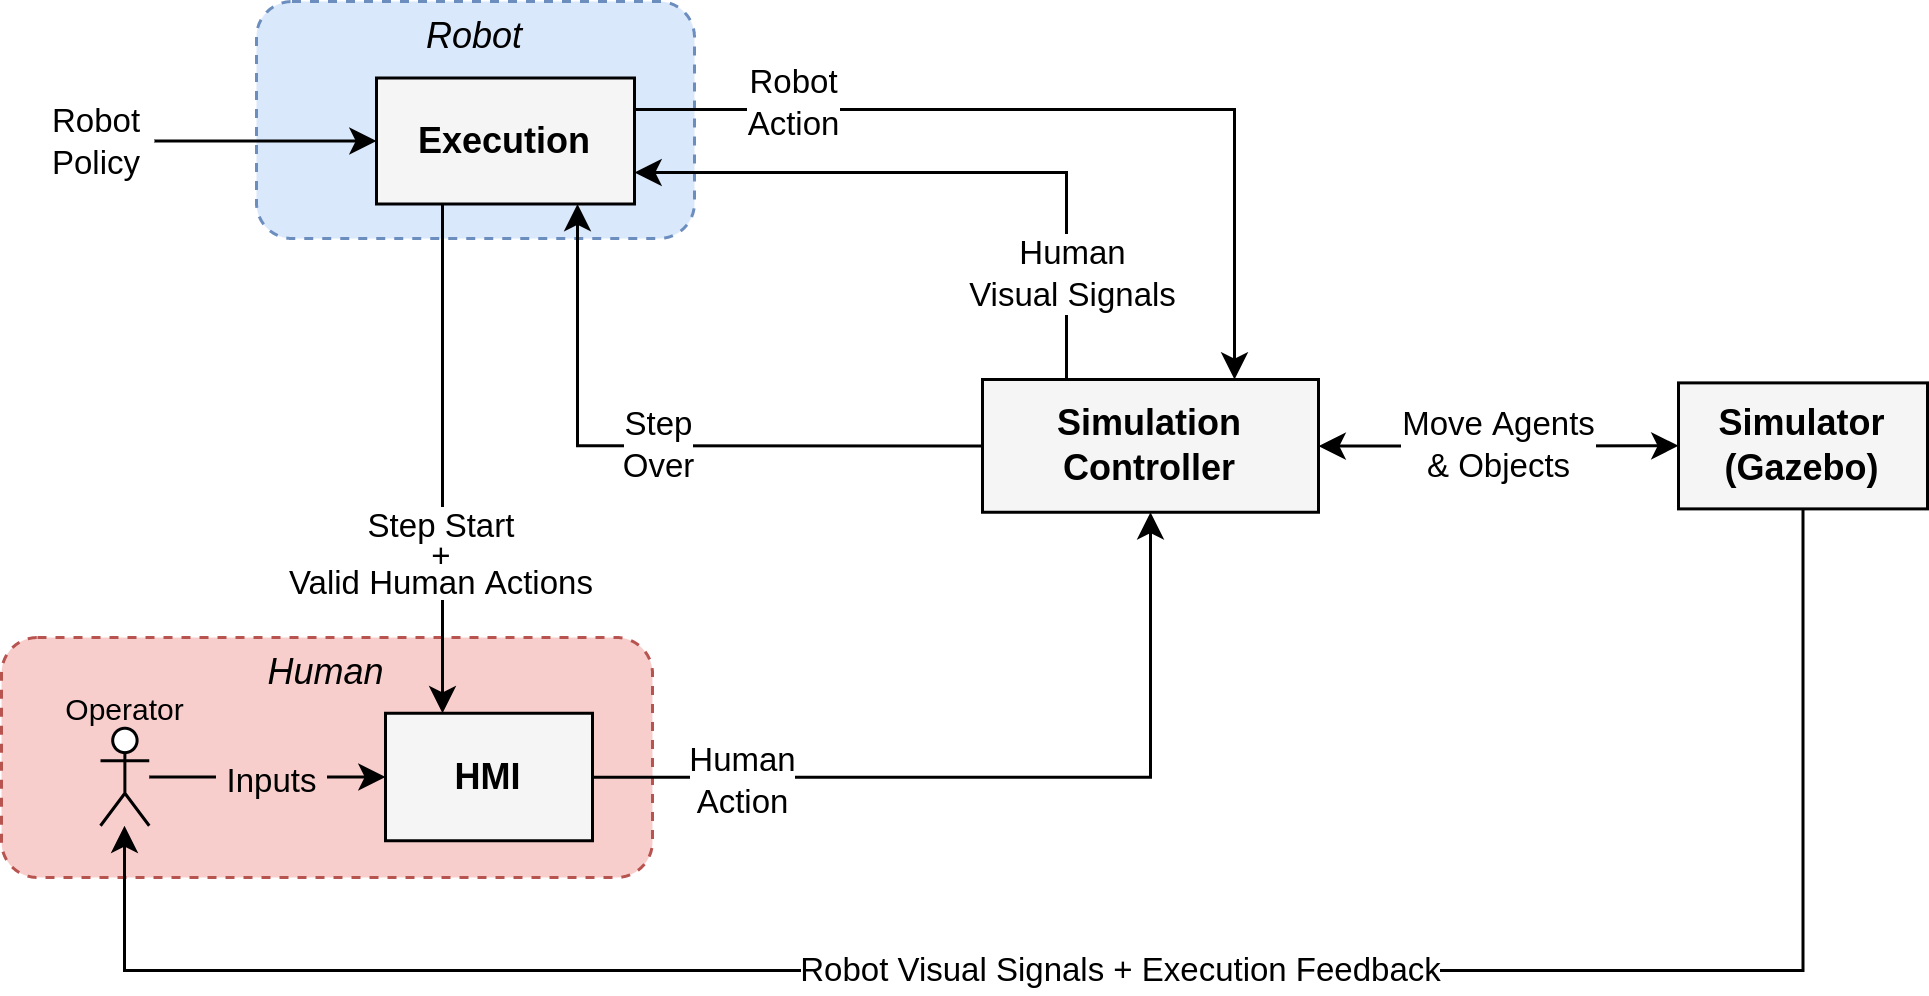
\includegraphics[width=\textwidth]{images/Chapter5/simulator.png}
    \caption{Interactive Simulator Overview}
    \label{fig:iteractive_simulator}
\end{figure}

\section{Study protocol}

objective, participants, material, experiment design, procedure, measures

This section describes the objectives and protocol of this study.  

\begin{figure}
    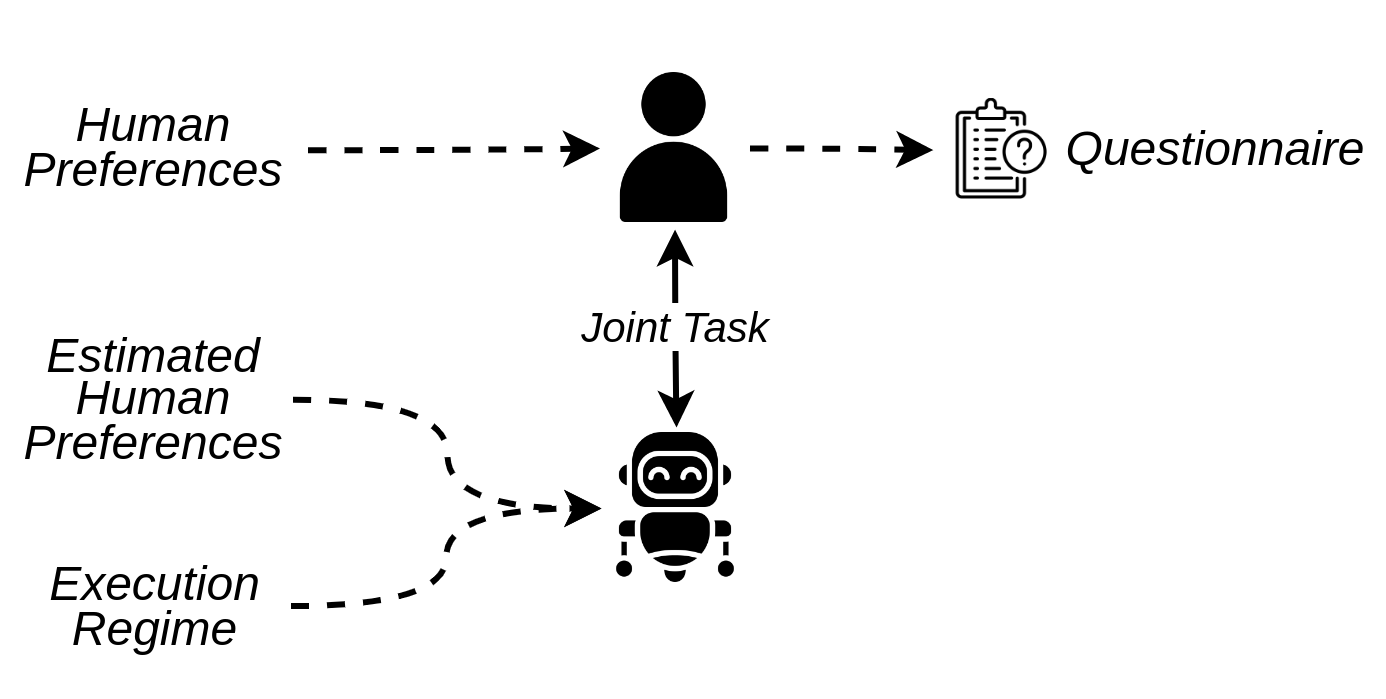
\includegraphics[width=\textwidth]{images/Chapter5/UserStudyProcedure.png}
    \caption{User Study Protocol. Each participant goes through 6 scenarios and answer 6 questionnaires to evaluate each different robot behavior}
    \label{fig:user_study_protocol}
\end{figure}




Through this study we want to demonstrate the benefits of using the model of execution described in the previous chapter~\ref{chap:4} in a collaborative context. We believe this model of execution is pertinent to be taken into account when executing and supervising a robot's plan. For the same reasons we based the policy generation of this model and aim to justify our choice and validate our approach.

In this study, each participant is made to collaborate six times with a simulated robot to achieve a shared task, each time is referred to as a scenario. The robot exhibits a different behavior in each scenario. After each scenario, the participant evaluate the robot's behavior through the PeRDITA questionnaire \cite{devin_evaluating_2018}.

Beforehand, every participant answers a few general/demographic questions and is familiarized with the simulator functionalities through an integrated tutorial. Only then they start the six consecutive collaborative scenarios, answering every time a questionnaire to describe the interaction. Eventually, every participant is asked to share their general feelings and impressions about the overall interaction with the simulated robot, and they are asked to tell which scenario they preferred the most and the least.

\begin{figure}
    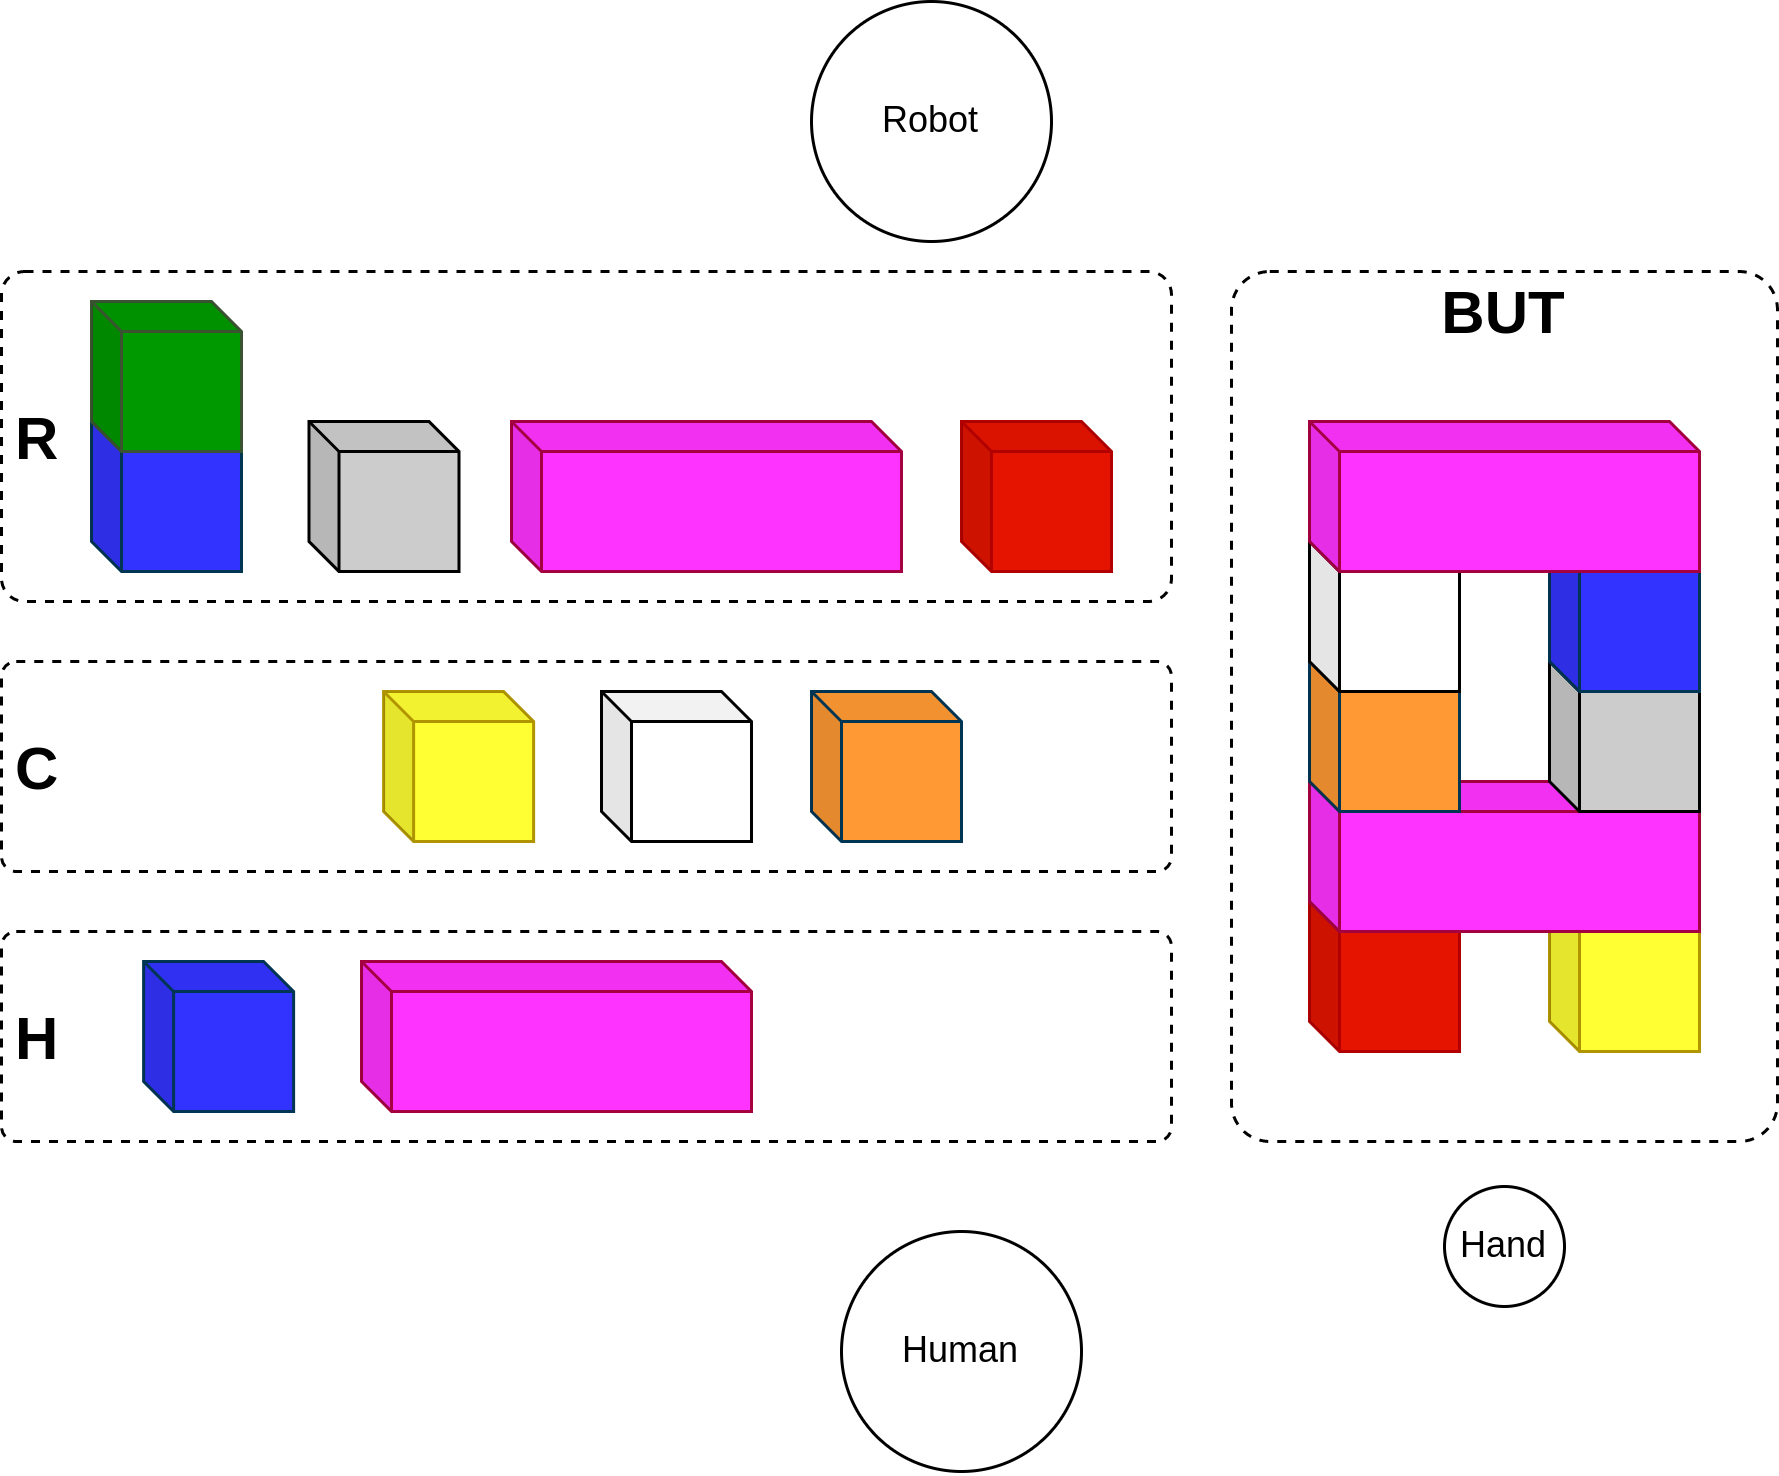
\includegraphics[width=\linewidth]{images/Chapter5/task_description_study.png}
    \caption{Description of the shared task to achieve in the study.}
    \label{fig:task_description_study}
\end{figure}

We now provide details about the task, the scenarios and how the different robot behavior are generated. 
The shared goal, which is stacking the cubes to match the given pattern, remains the same in all scenarios. The cube disposition on the table also doesn't change either. The task description is depicted in fig~\ref{fig:task_description_study}. 

To progress in the task, the agents can perform three different primitive actions which are the following: \textit{pick} a cube, \textit{place} a cube in the stack, or, \textit{drop} a cube back on the table.
These actions have a few preconditions, more or less intuitive, that are communicated and experienced by the participant during the integrated tutorial.
First, one can \textit{place} a cube if they hold the cube, and if the targeted location is free and supported. That is, the cubes directly below the targeted location must be placed before being able to place a cube in the targeted location.
Secondly, one can only \textit{pick} a cube from their respective reachable zones of the table, i.e., Human and Center zones for the human, and Robot and Center zones for the robot. Also, one can only pick a cube if it can be placed immediately. Thus, one cannot pick a cube ``in advance'' and has to wait to its placement condition to be true before picking it up. For instance, both pick bars can only be picked up after the yellow and red cubes have been placed. This rule helps to create interaction conflicts serving the purpose of this study. Moreover, although the participants find this not intuitive they get used to it really fast and this feeling seems to be significantly reduced along the experiment.
Third, one can \textit{drop} a cube back on the table only if they hold it and if it cannot be placed.

For each scenario the participant is given instructions regarding how to solve the task. The participants are asked to consider these instructions as their own choice and preferences regarding the task resolution, and thus, to act accordingly while collaborating. The instructions at each scenario are one of the two following.
On the first hand, the participant shall act in a way to finish the task as soon as possible. Here, it consists in trying to perform as many actions in parallel as possible to progress faster. These preferences are latter referred to as Task End Early (TEE).
On the other hand, the participant shall act in a way to be freed as soon as possible. That is, they should finish their mandatory part of the task as soon as possible, so they could leave and let the robot finish alone. Here it consists in placing the pink bar from the Human zone as soon as possible. These preferences are latter referred to as Human Free Early (HFE).
On its side, the robot doesn't directly have access to these instructions/preferences, they are only estimated. Hence, for each scenario, the robot is given a more or less accurate estimation of the human preferences that are communicated to the participant. Note that the participants aren't aware that the robot has an estimation of their preferences, neither that this estimation can be inaccurate.
This way, we created three scenarios with different pairs of human preferences and associated estimation. In the first pair, the human shall finish the task early and the robot has a correct estimation, i.e., the robot's policy is helping the human to finish the collaborative task early. In the second pair, the human preferences remain the same, but the robot estimation is incorrect. The robot is trying, mistakenly, to minimize the human effort. As a consequence, the robot tends to pick cubes that the human could pick, preventing the human from acting and making the task completion longer. In the third pair, the human shall free themselves early, but the robot estimation is again erroneous. The robot will try to finish the task early while its priority is to place the first pink bar, which is conflicting with the given human preferences.

Additionally, in each scenario, the robot follow one of the two following execution regimes:
\begin{itemize}
    \item \textbf{Robot-First (RF)}: the robot always initiates actions first, and the participant take action afterwards.
    \item \textbf{Human-First (HF)}: the robot always lets the participant take the initiative, and then acts.
\end{itemize}
The \textit{Human-First} execution regime corresponds to the Model of Execution described in the previous chapter. At each step, the robot waits for the human's decision and will execute the best action that complies with it. The human always start acting first and the robot follows. On the other hand, the \textit{Robot-First} regime corresponds to a naive and straightforward policy execution where, at each step, the robot directly starts executing the overall best robot action given by the policy. The robot always starts acting forcing the human to comply. The \textit{Robot-First} regime serves as a baseline to evaluate the proposed \textit{Human-First} regime, described by our Model of Execution and used in the policy generation.
Eventually, we associate each of the three previous pairs of preferences and estimation with one of the two different execution regime. As a result, we obtain six different scenarios with six different robot behaviors named in table~\ref{tab:scenario_names}.

\begin{table}
    \caption{Name of the six scenarios. 
    Columns represent the preferences/estimation pairs and the rows correspond to the execution regimes.}
    % \vspace{-15pt}
    \begin{center}
    \begin{tabular}{c|c|c|c|}
        \cline{2-4}
        & TEE: correct  & TEE: incorrect    & HFE: incorrect\\
        \hline
        \multicolumn{1}{|c|}{Human-First}     & S1            & S2                & S3\\
        \hline
        \multicolumn{1}{|c|}{Robot-First}     & S4            & S5                & S6\\
        \hline
    \end{tabular}
    \end{center}
    \label{tab:scenario_names}
\end{table}

Note that our goal is to evaluate and compare the different robot behaviors. However, at the beginning, the participants don't have any references to compare with which can influence their answers in the very first scenarios. One solution is to ask the participants to answer all six questionnaires at the end, after being familiar with the six scenarios. We consider that this option demands a too heavy mental workload to recall accurately each specific scenario, and may bias the answers. As a consequence, we decided to ask the participants to answer the questionnaire after each scenario as a draft. Along the experiment, they can rectify their answers to match more accurately their feelings. At the end, using the drafts, they share their final answers for each scenario. We believe this process allow to more accurately gather the feelings of the participants. Moreover, the ordering in which the participants encounter the scenarios is uniformly randomized to prevent any order effect. 

\textbf{TODO: Give more details about the PeRDITA questionnaire (questions, goal, etc..)}

On top of the answered questionnaires, for each scenario, the interactive simulator produces logs from which we extract several metrics and an overall timeline of the execution. The timeline depicts the activities and actions of each agent along the task progression. The subjective measures done through the questionnaire are complemented with the objective metrics extracted such as the duration to complete the task, the number of human action, the total duration of human inactivity, and more. 



\section{Study results}

In this section, we share the main results obtained through the answered questionnaires and the metrics extracted from the logs.



\subsection{From timeline}
\textbf{TODO: For now with only 9 participants, it is hard to extract any relevant result from the logs. The timelines vary considerably. So far, we can say that S2 seems faster than S1. And aberrant result can be found in certain scenarios. However, we also extract the ratio of optimal human action, depicting if the participant followed optimally or not the given instructions. This metric helps to justify this aberrant results since the participant behaved significantly differently than the others.}

\subsection{From questionnaires}

Some questions have large standard deviation, such as about the perceived ``Intelligence'', but often only on specific scenarios.

The ``Reactive'' answers are overall the same, whatever execution regime and scenario. 
Overall, based on an ANalysis Of the VAriance with repeated measures (ANOVA), all other answers than ``Reactive'' vary significantly. Post tests show that the main differences come from the scenarios S4 and S6. Those two scenarios correspond to ones where the robot has an incorrect estimation of the human preferences and is following the \textit{Robot-First} execution regime. This indicates that all HF behaviors are perceived similarly despite the erroneous estimation of the robot. It also indicates that the RF scenario with correct estimation is positively perceived, but an erroneous estimation has significant impact on the answers when using RF.  

Except the ``Reactive'' aspect, answers about RF have larger standard deviation. Thus, participants tend to be more indecisive regarding RF than HF.

We notice very few significant differences on HF only.

\begin{figure}
    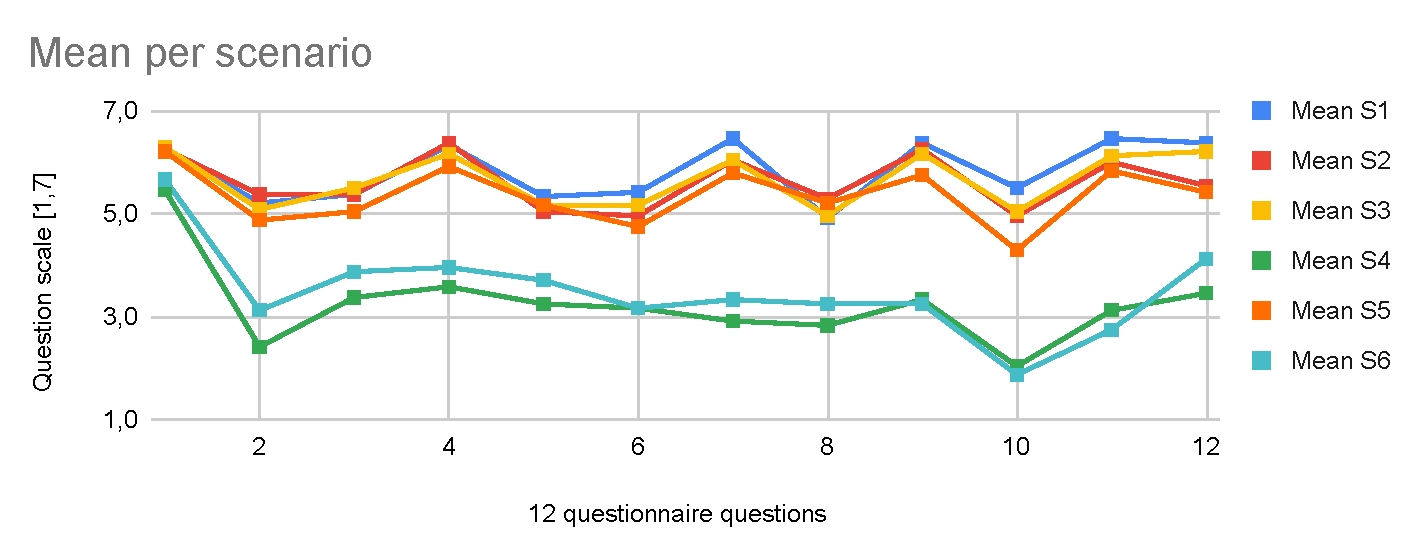
\includegraphics[width=\linewidth]{images/Chapter5/Mean per scenario.pdf}
    \caption{Mean answers per scenario}
    \label{fig:mean_per_scenario}
\end{figure}

\begin{figure}
    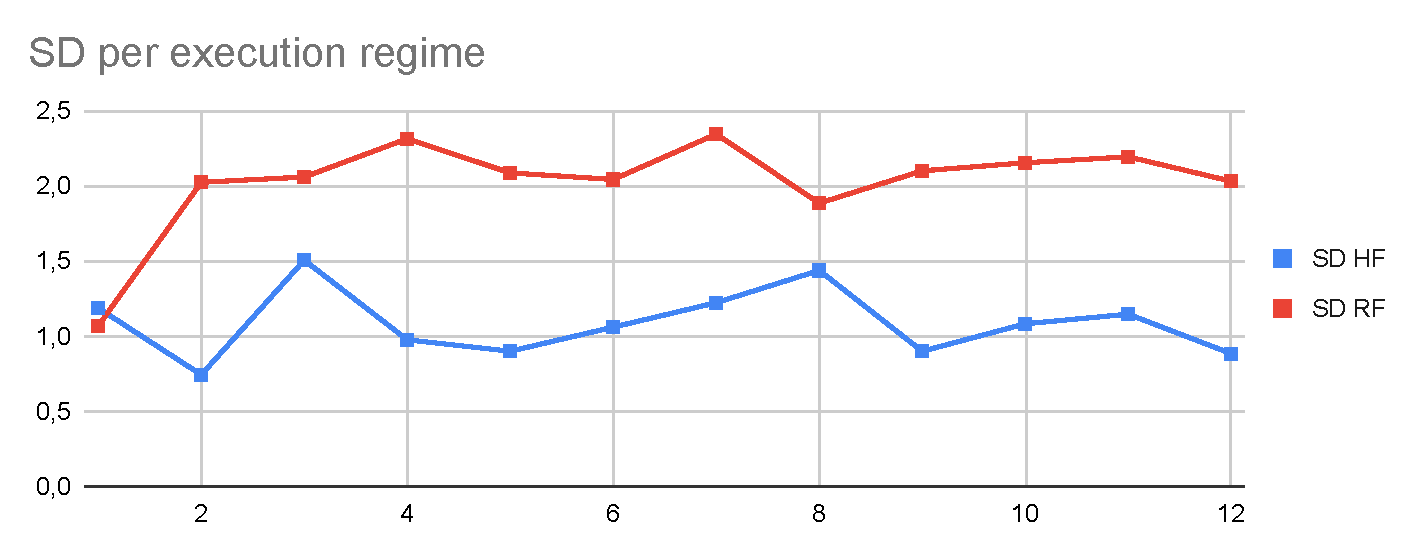
\includegraphics[width=\linewidth]{images/Chapter5/SD per execution regime.pdf}
    \caption{SD per Execution Regime}
    \label{fig:sd_per_execution_regime}
\end{figure}


\section{Discussion}



\section{Conclusion}

